\documentclass{article}
\usepackage[utf8]{inputenc}
\usepackage{graphicx}
\usepackage{hyperref}

\title{Lab 03- ARP Poisoning and DHCP Security}
\author{Matthew Belanger}
\date{\today}

\begin{document}

\maketitle

\newpage

% SECTION 1

% TASK 1

\section{Task 1: ARP Poisoning Attack}
\label{sec:task1}

\section*{Tasks}

\subsection{\textbf{Environment Setup}: Create a simple network with two virtual machines (VM1 and VM2) connected
through a virtual switch or host-only network. Ensure both VMs can ping each other, confirming
network connectivity.}

See Figure \ref{fig:connected}

\begin{figure}[h]
    \centering
    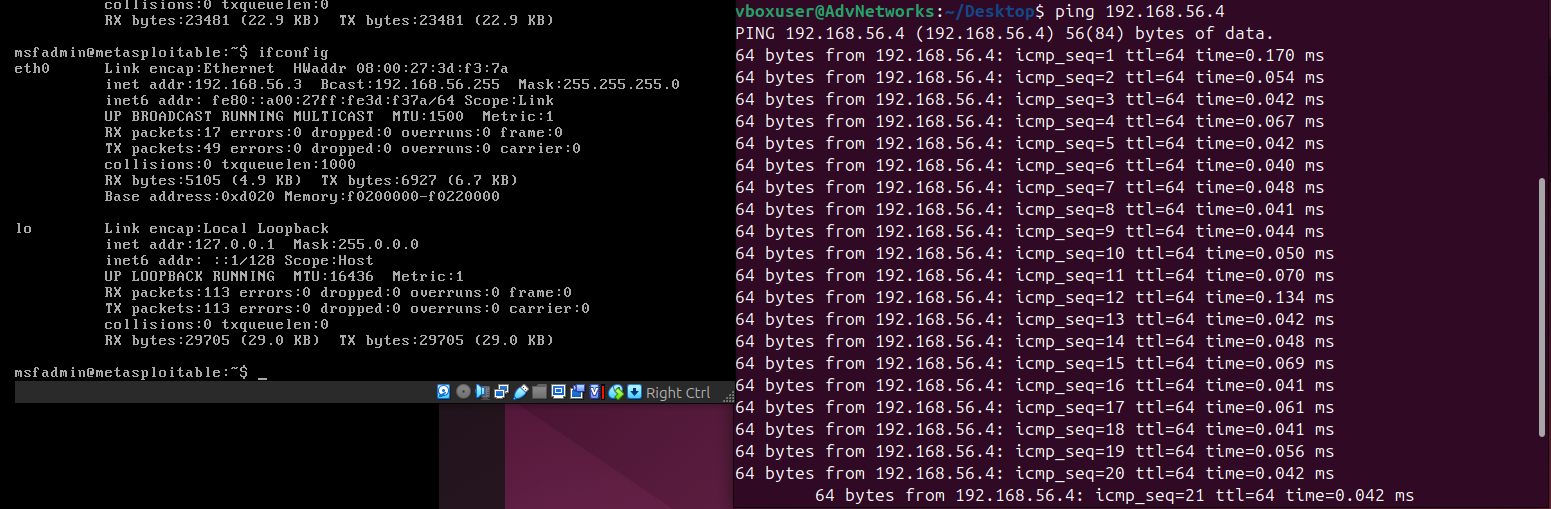
\includegraphics[width=0.8\textwidth]{task1/screenshot/connected.png}
    \caption{VMs Connected}
    \label{fig:connected}
\end{figure}


\subsection{\textbf{ARP Security Testing}: Write a script using Scapy to perform ARP security testing (pentesting), follow the STRIDE methodology we applied in the class to test and verify the identified vulnerabilities.}

See code \href{https://github.com/MattBelanger321/COMP8670/tree/master/lab3/task1}{Repo}

\subsection{\textbf{Mitigation and Report}: Discuss and implement basic mitigation strategies against ARP poisoning,
such as static ARP entries or using ARP spoofing detection tools.}

\label{subsubsec:arp-mit}

\section*{Report Requirements}

\subsection*{Network configurations and ARP tables before and after the attack.}

\subsubsection*{Before}

See Figure \ref{fig:before}

\begin{figure}[h]
    \centering
    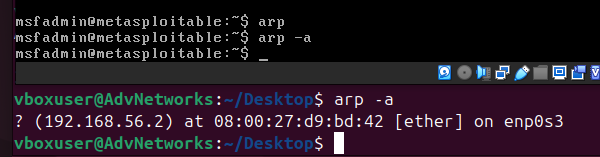
\includegraphics[width=0.8\textwidth]{task1/screenshot/before.png}
    \caption{VMs Connected}
    \label{fig:before}
\end{figure}

\subsubsection*{After}

See Figure \ref{fig:after}

I am pretending to be the DHCP server here. You can see the ARP table has two IPs with the same MAC. 

\begin{figure}[h]
    \centering
    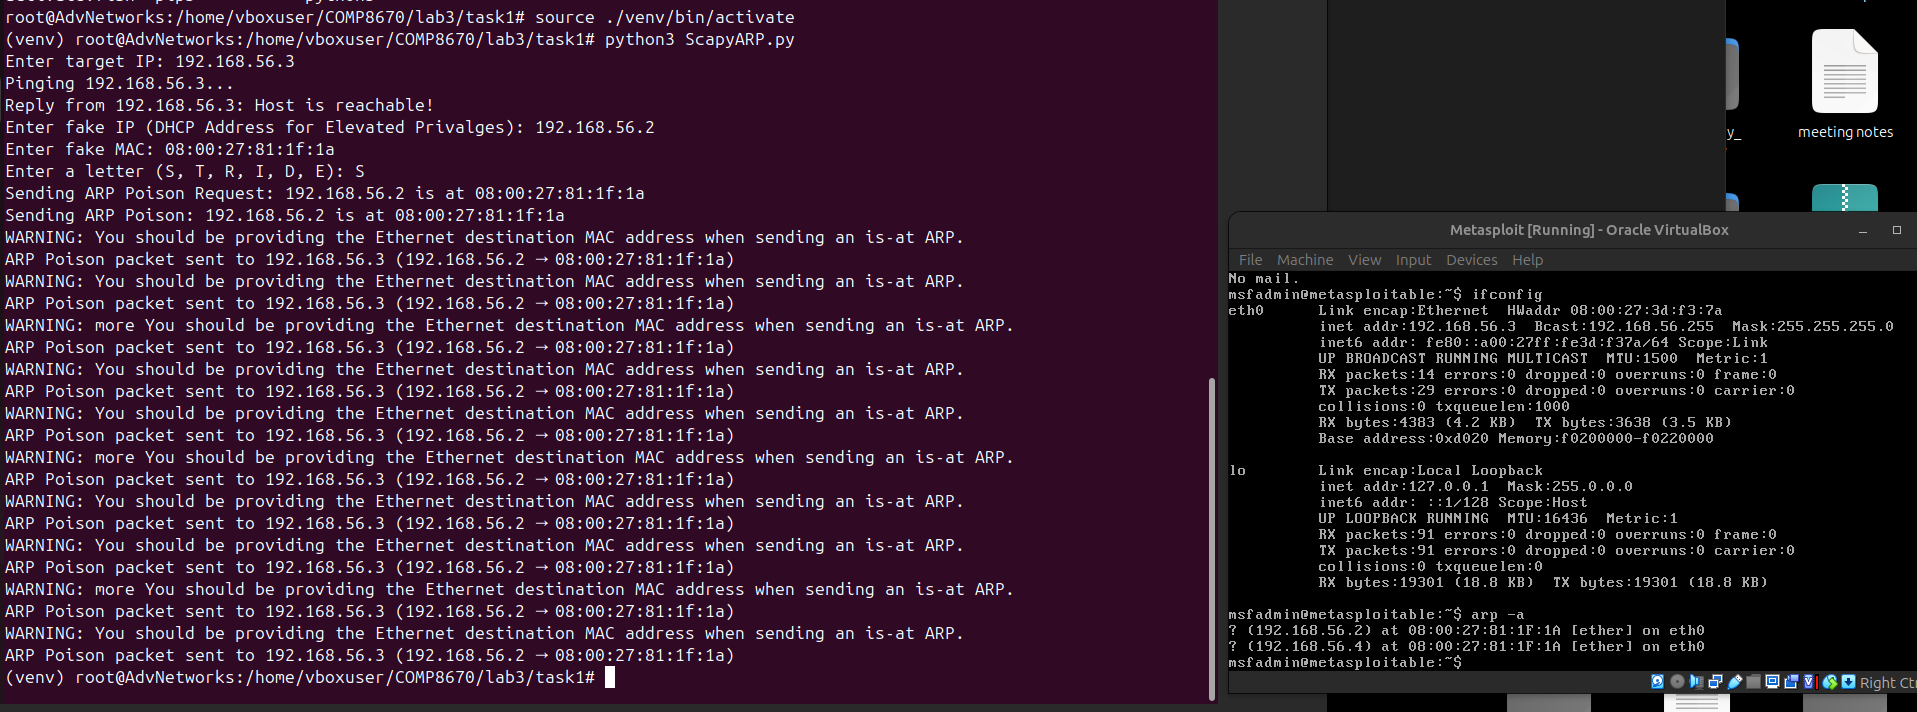
\includegraphics[width=0.8\textwidth]{task1/screenshot/poison.png}
    \caption{Poisoning Screenshot}
    \label{fig:after}
\end{figure}

\subsection*{Scapy scripts used.}

See code \href{https://github.com/MattBelanger321/COMP8670/tree/master/lab3/task1}{Repo}

\subsection*{Screenshots demonstrating the success of the attack, including Wireshark captures.}

In figure \ref{fig:wireshark-proof} I pretend to be the DHCP server at 192.168.56.2 (actual IP 192.168.56.4). On the victim machine I ping the DHCP server but the packets are recieved on hackers machine.

\begin{figure}[h]
    \centering
    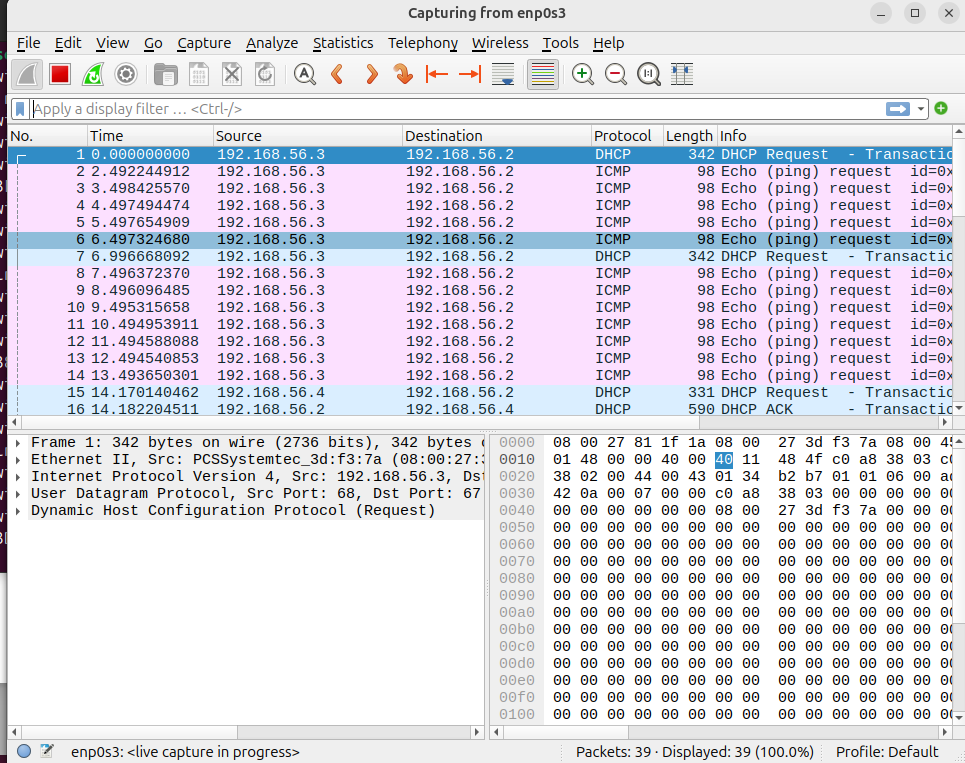
\includegraphics[width=0.8\textwidth]{task1/screenshot/wireshark_spoof_proof.png}
    \caption{Wireshark Spoof}
    \label{fig:wireshark-proof}
\end{figure}

\subsection*{Discussion on mitigation strategies.}

See section \ref{subsubsec:arp-mit}

\newpage

% TASK 2

\section{Task 2: Security Analysis of The DHCP}

\subsection{Start Wireshark open the enclosed pcap trace file and list all the DHCP packets in the trace. Use
screenshots to support your answer.}

See Figure \ref{fig:pcap_dhcp}

\begin{figure}[h]
    \centering
    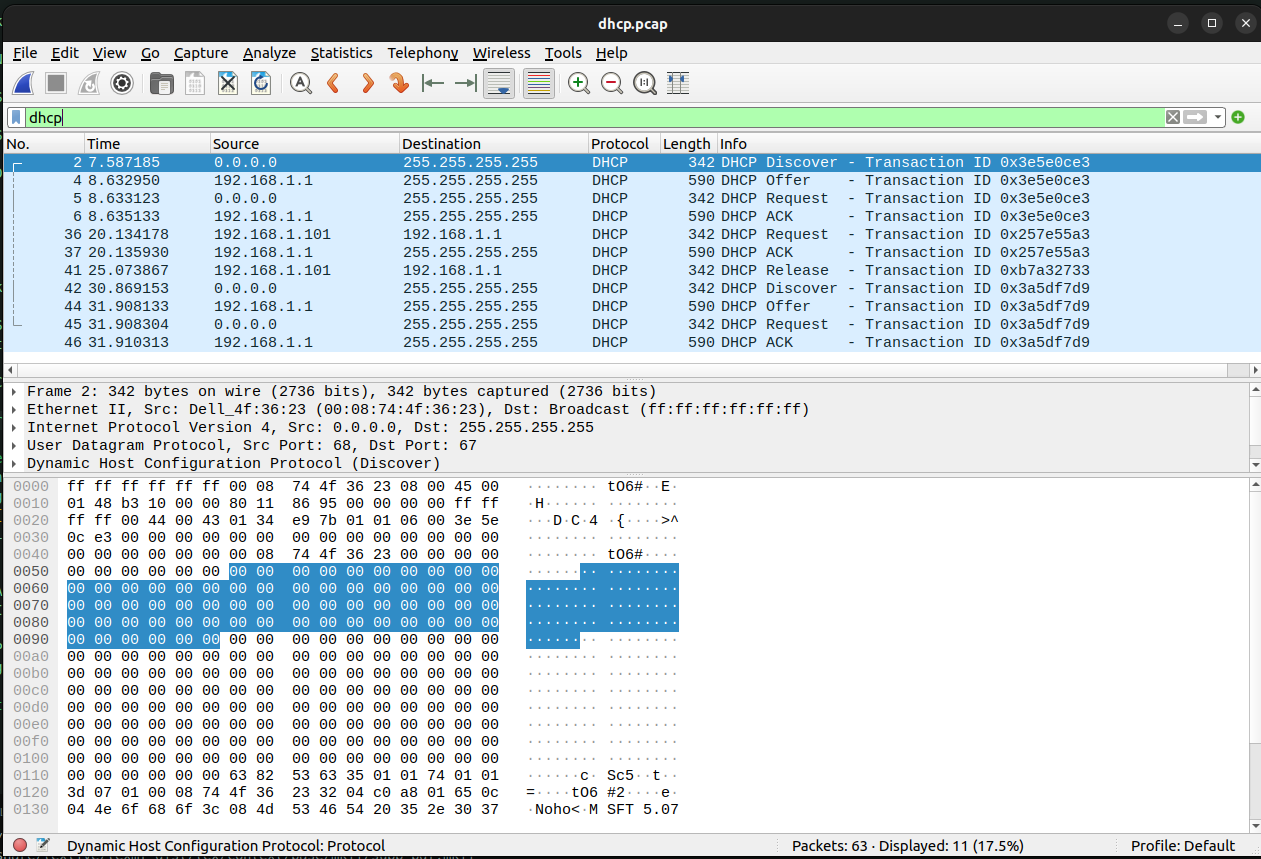
\includegraphics[width=0.8\textwidth]{task2/dhcp_wireshark.png}
    \caption{DHCP Packet List}
    \label{fig:pcap_dhcp}
\end{figure}

\subsection{Create a Finite State Machine model for the DHCP process.}
 
See Figure \ref{fig:dhcp_fsm}

\begin{figure}[h]
    \centering
    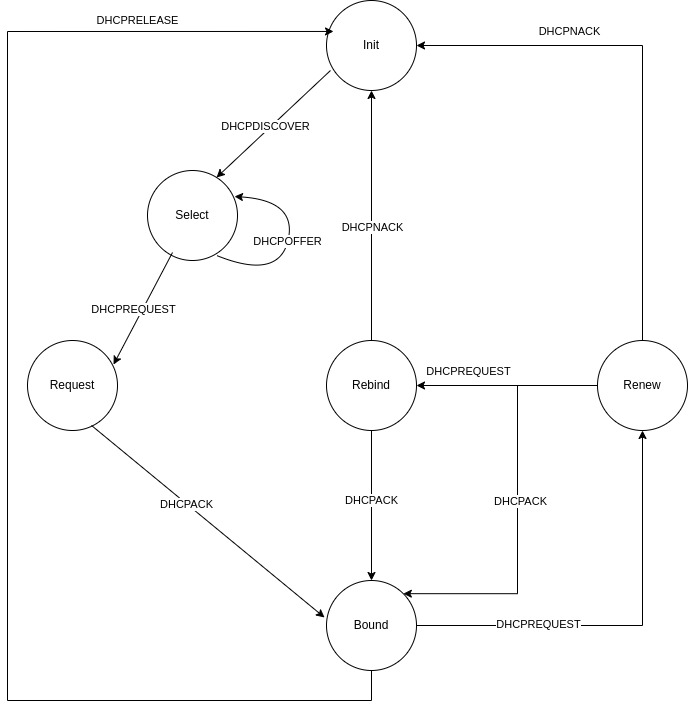
\includegraphics[width=0.8\textwidth]{task2/DHCP_FSM.jpg}
    \caption{DHCP Finite State Machine}
    \label{fig:dhcp_fsm}
\end{figure}

\subsection{Apply the STRIDE methodology to the FSM model of DHCP to identify potential security threats.
For each STRIDE element, identify possible vulnerabilities in the DHCP process.}

\subsubsection{Spoofing}

\subsubsection{Tampering}

\subsubsection{Repudiation}

\subsubsection{Information Disclosure}

\subsubsection{Denial of Service}

\subsubsection{Elevation of Privilege}

\subsection{Propose mitigation strategies for each identified vulnerability. This could involve protocol enhance-
ments, configuration changes, or additional security mechanisms.}

\subsubsection{Spoofing}

\subsubsection{Tampering}

\subsubsection{Repudiation}

\subsubsection{Information Disclosure}

\subsubsection{Denial of Service}

\subsubsection{Elevation of Privilege}

\end{document}
